\chapter{Evaluation} \label{chap:evaluation}

In the previous chapter, \S\ref{chap:system}, we have presented our implementation of live migration of containers using \criu and \runc, and have motivated our design choices with micro-benchmarks that fulfil the initial objectives specified in the introduction.
In this chapter, we move on to evaluate the system as a whole, and how the different features interlace and work together, and  how does our system compare to traditional virtual machine live migration.

In all the experiments here presented, and unless otherwise stated, we use the same experimental setup than in the micro-benchmark chapter.
Two (if necessary) Linux Debian machines with kernel version $4.19.0-6$ running on a host-only network in VirtualBox version $5.2.34$.
\criu version $3.13$ and \runc version $1.0.0-rc8$, both built from source.

\section{Application Downtime}

In this section we study the impact of the threshold value we set to stop the iterative migration and dump the application in the total downtime.
As previously introduced in the \textit{Iterative Migration} section from \S\ref{sec:arch-blocks}, we establish an arbitrary parameter to decide when to stop transferring only memory dumps (\textit{i.e.} pre-dumping the container process) and checkpoint, hence freeze, and migrate the application to the remote host.
A reasonable rule of thumb is to establish a memory cap, and whenever the successive dumps are smaller than said cap, trigger the threshold and exit the loop.
However, a hard-coded value would be very ad-hoc to our experimental setup.
Therefore, we have benchmarked the impact of setting a variable memory cap to the total downtime.
The values we choose are proportional to the size of the initial allocated memory pool.

In order to test this feature we set up the following experiment.
We deploy an in-memory \textsc{Redis} database with 1e6 keypairs which result in an allocated memory (for all the container) of several hundreds of MB.
We use \texttt{redis-client} and \texttt{redis-server} version $5.0.3$.
For each run, we set a percentage of the initial memory as our threshold value, and report the total application downtime and a breakdown of the time spent (in percentage) during the last dump of each iteration.
In particular we measure the time spent dumping the memory (\texttt{dump}), preparing the migration (\texttt{prepare}), transferring files to the other host (\texttt{transfer}) and during restore (\texttt{restore}).
We present our results in Figure~\ref{fig:downtime}.

\begin{figure}[h!]
    \centering
    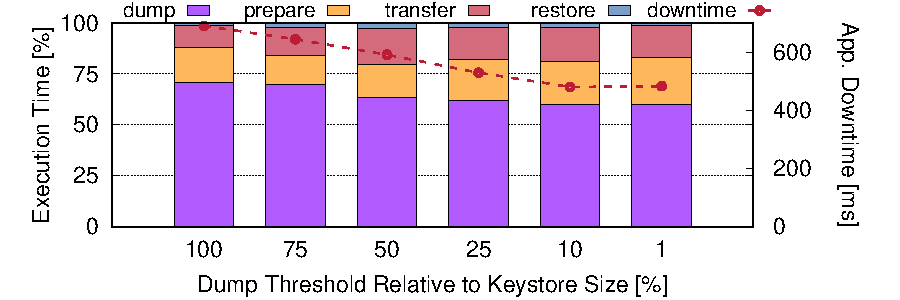
\includegraphics[width=\textwidth]{./figs/downtime/downtime.pdf}
    \caption[Application Downtime Relative to Threshold]{Application downtime relative to the memory threshold cap (dotted red), and stacked histogram of the time spent in each phase during the last dump.\label{fig:downtime}}
\end{figure}

We observe that, for our particular setting, once the memory cap reaches $10\%$ of the original size, the application downtime reaches the baseline value.
Moreover it is also interesting to see that, as this value gets closer to the baseline, the time spent (absolute and relative) dumping memory decreases.
This results are specific to our setting with two virtual machines and limited memory, but a similar benchmark could be reproduced in production to estimate an adequate threshold value.

\section{Memory Scalability}

In this section we study the scalability of our approach with respect to the memory allocated by the to-be checkpointed container.
For this experiment we set up a \textsc{Redis} in-memory database which we pre-load with a variable number of key-value pairs.
We use, similarly to the previous section, \texttt{redis-client} and \texttt{redis-server} version $5.0.3$, and pre-load the keys using the \texttt{--pipe} flag for bulk data upload.
In Listing~\ref{code:redis-bulk-upload} we include the script for doing so.
Note that this same strategy was also used in other benchmarks using \textsc{Redis}.
\begin{lstlisting}[style=Bash,caption={Snippet for bulk data upload to a Redis database.},label={code:redis-bulk-upload}]
#!/bin/bash

# Start a runc container named redis-db
# The ip the service runs on is stored in the .ip file
sudo runc run -d redis-db &> /dev/null < /dev/null

# Populate DB with data
cat "./data/file.dat" | redis-cli -h `< .ip` --pipe
\end{lstlisting}

Our goal is to evaluate the impact of the size of the memory allocated to the overall container downtime.
In order to compare against a naive live migration (checkpoint, transfer files, and restore on the remote end) and traditional virtual machine migrations, we choose not to use iterative migration in our system.
This is due to the fact that it would be an unfair advantage against the other two systems.
Additionally, and in order to avoid noise introduced by the network latency, we run migrations locally (\textit{i.e.} transfering files to $127.0.0.1$).
We measure the application's downtime (time to checkpoint plus time to restore) when running an in-memory \textsc{Redis} database pre-loaded with key-value pairs of sizes raging $16 B$ for one pair to $265 MB$ for $1e7$ pairs.

\textbf{Comparison Against Naive Live Migration.}

We first compare against a \textit{naive} live migration.
We define by \textit{naive} the process of dumping (hence stopping) a process, transferring the dump files, and restarting it in the remote end.
We report the downtime for this approach and our system when ran with only one iteration in Figure~\ref{fig:key-scalability}.
\begin{figure}[h!]
    \centering
    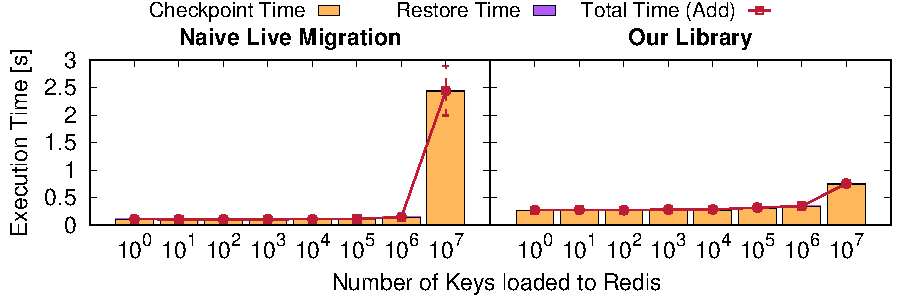
\includegraphics[width=\textwidth]{figs/key-scalability/key_scalability.pdf}
    \caption[Scalability with respect to the memory to transfer.]{Scalability with respect to the memory to transfer. We compare our system with manual live migration when running in the same machine with a one-shot migration.\label{fig:key-scalability}}
\end{figure}

From our results we are able to extract different conclusions.
First of all, the time to restore is negligible when compared to the time to checkpoint/dump the container.
Secondly, even though our library introduces a small overhead, around $0.1$ seconds, to the baseline, this proofs efective in the long run when the application downtime is reduced by a factor of five.
Lastly, we also observe that a user will specially benefit from using a specialized live migration library like ours over the manual approach whenever the container to checkpoint is resource-eager.

\textbf{Comparison Against Virtual Machine Migration}

In this second comparison, we compare against traditional virtual machine migration.
Given that our test nodes were already running in VirtualBox version $5.2.3$, we have opted to use VirtualBox's native live migration solution: teleporting~\cite{vbox-teleport}.
From the user manual we read that teleporting boils down to moving one virtual machine from one VirtualBox host to another one over TCP/IP.
In our particular experiment, the VirtualBox  host would be the same, as we are migrating to \texttt{localhost}, but to a different virtual machine (a pre-made clone of the origin one).
In Listing~\ref{code:vm-teleport} we include the evaluation snippet we used to launch the experiments and teleport the machines.
Note that some additional commands had to be made through the GUI, and that the \texttt{./run\_redis.sh} script is very similar to the one presented in Listing~\ref{code:redis-bulk-upload}.

\begin{lstlisting}[style=Bash,caption={Script to teleport a VirtualBox VM, and run the macrobenchmark.},label={code:vm-teleport}]
#!/bin/bash

# Configure target machine to wait for a teleport request to arrive
VBoxManage modifyvm 'CRIU-Debian-Teleport-Target' --teleporter on --teleporterport 6000

# Iterate over the different number of keys
for num_keys in 1 10 100 1000 10000 100000 1000000 10000000
do
    # Start the host machine as usual
    ssh <HOST_VM>
    cd ~/runc-containers/redis && ./run_redis.sh 100000

    # Start the target machine, if using a normal start, a process dialog will appear

    # Run the migration
    time VBoxManage controlvm 'CRIU-Debian' teleport --host localhost --port 6000

    # Shut down both VMs
done
\end{lstlisting}

We present our results in Figure~\ref{fig:vm-teleport}.
The first observation we can make, is that VM live migration has a significantly higher overhead in the baseline case.
This was to be expected as overall overhead and slow boot times are the main argument in favour of containers and against virtual machines.
And in this experiment we are running one inside of the other.
However, what is also worth noticing is the scalability.
Whilst our system (for which we re-plot the same results from Figure~\ref{fig:key-scalability}), experiences an increase in downtime of $\times 1.5$, VirtualBox's experiences a downtime closer to $\times 2$ (whilst naive migration had one closer to $\times 10$).
This result shows that, even with a drastically smaller overhead, our system also showcases a better scalability when compared to traditional VM migration.

\begin{figure}[h!]
    \centering
    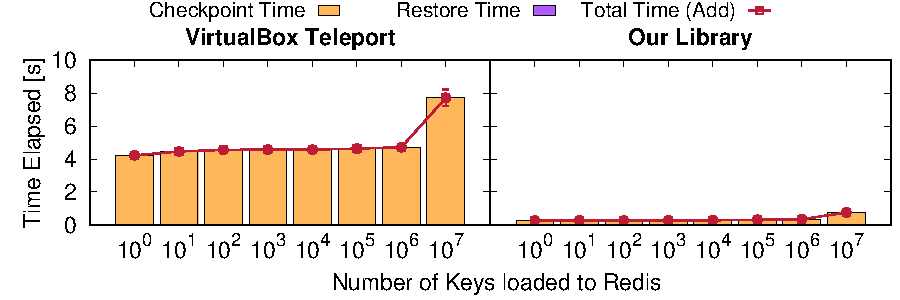
\includegraphics[width=\textwidth]{figs/vm-teleport/vm_teleport.pdf}
    \caption[Scalability comparison with VirtualBox Teleport.]{Scalability with respect to the memory to transfer. We compare our system with VM live migration using VirtualBox's Teleport functionality.\label{fig:vm-teleport}}
\end{figure}
